\documentclass[11pt]{article}
\usepackage{graphics,epsfig,amsmath,amssymb}
\usepackage{epsf}
\usepackage{boxedminipage}
\usepackage{fullpage}
\usepackage{fancyheadings}
\usepackage{times}
\usepackage{amsmath}
\usepackage{ifthen}
%\usepackage{pseudocode}
\usepackage{psfrag}
\pagestyle{fancy}

\setlength{\topmargin}{.2in}
\setlength{\parindent}{0in}
\setlength{\parskip}{.15in}
\setlength{\footskip}{0.1in}

\newcounter{pctr}
\stepcounter{pctr}

\newcounter{partctr}

\newcommand{\ie}{{\em i.e.}}
\newcommand{\eg}{{\em e.g.}}

\newcommand{\ch}{\item {\bf True~~/~~False~~}}
\newcommand{\tfnote}{\probnote{Circle True or False for each choice.}}
\newcommand{\allapply}{\probnote{Circle ALL that apply}}
\newcommand{\bestanswer}{\probnote{Circle the BEST answer}}
\newcommand{\ansbelow}{\probnote{Answer legibly in the space below.}}

\renewcommand{\thesection}{{\bf\Roman{section}}}
\renewcommand{\theenumi}{{\bf\Alph{enumi}.}}
\renewcommand{\labelenumi}{{\bf\Alph{enumi}.}}

\newcommand{\setversion}[1]{\def\version{#1}}
\setversion{quiz}

\ifthenelse{\equal{\version}{answers}}{
    \newcommand{\sols}[1]{#1}
} {
    \newcommand{\sols}[1]{}
}


\newcounter{answer}
\newenvironment{answer}[1][\relax]{\refstepcounter{answer}\begin{list}%
 {}{\leftmargin 0pt\rightmargin 0pt\labelsep 3pt\parsep 0pt%
 \setlength{\listparindent}{\parindent}}
    \item {\bf Answer \theanswer #1}\
    }{\hspace*{\fill}$\blacksquare$\end{list}} 



% uses these macros to delimit problems
\newcommand\prob[1]%
  {\begin{itemize}\item[]%
   \vspace{.2in}{\bf\thepctr. ~[#1~ points]:}\stepcounter{pctr}}
\newcommand\eprob{\end{itemize}}
\newcommand\probnote[1]%
  {\\\begin{tabular}{cr} \hspace{3in} & {\bf (#1)} \\ \end{tabular}}

% headers/footers
\lhead[\fancyplain{}{\bf Page \thepage ~of \pageref{lastpage}}]%
      {CS 6262 Spring 2009, Quiz 1}
\lfoot[{\bf Initials: }]%
      {{\bf Initials: }}
\rhead[CS 6262 Spring 2009, Quiz 1]%
      {\fancyplain{}{\bf Page \thepage ~of \pageref{lastpage}}}
\cfoot{}
\setlength{\headrulewidth}{0in}
\setlength{\headsep}{.3in}

 % Compact itemize and enumerate.  Note that they use the same counters and
% symbols as the usual itemize and enumerate environments.
\def\compactify{\itemsep=0pt \topsep=0pt \partopsep=0pt \parsep=0pt}
\let\latexusecounter=\usecounter
\newenvironment{CompactItemize}
  {\def\usecounter{\compactify\latexusecounter}
   \begin{itemize}}
  {\end{itemize}\let\usecounter=\latexusecounter}
\newenvironment{CompactEnumerate}
  {\def\usecounter{\compactify\latexusecounter}
   \begin{enumerate}}
  {\end{enumerate}\let\usecounter=\latexusecounter}

\begin{document}
\cfoot{}
\pagestyle{empty}

\vspace*{-0.2in}
\begin{center}
\begin{tabular}{lr}
\resizebox{1in}{!}{
\includegraphics{GT}}
&
\parbox{4in}{
    {\Large\it College of Computing} \\ \\
    {\LARGE\sf Georgia Institute of Technology} 
}
%
\end{tabular}
\end{center}

\begin{center}
{\Large{\bf CS 6262: Network Security: Spring 2009} \\
 \vspace{.15in} \Huge{\bf Quiz I}} 
\vspace{.2in}

% this is the box on the first page with overall quiz information
\begin{boxedminipage}[h]{6in}
There are \underline{13 questions} and
  \underline{\pageref{lastpage} pages} in this quiz booklet (including
  this page).  Answer each question according to the instructions given.
  You have {\bf 85 minutes} to answer the questions.

%\vspace{.1in} The last page is an easy question.  {\em Rip this
%page off of your exam for five bonus points.}  Turn it in anonymously if
%you like.


\vspace{.1in} 
If you find a question ambiguous, write down any
assumptions you make.  {\bf Be neat and legible.}  If I can't
understand your answer, I can't give you credit!  There are three pretty
challenging questions (clearly marked); you may want to look through the
whole quiz and save those for last.

\vspace{.1in} 
Use the empty sides of this booklet if you need scratch space.  You
may also use them for answers, although you shouldn't need to.  {\em If you
do use the blank sides for answers, make sure to clearly say so!}

\vspace{.1in} 
{\bf Note well: Write your name in the space below AND your initials at the bottom of each
page of this booklet.}

\begin{center}{\bf THIS IS AN ``OPEN NOTES, OPEN PAPERS'' QUIZ.\\
LAPTOPS ARE ALLOWS, BUT NETWORKING IS NOT. \\
NO ENCRYPTED WIRELESS TRAFFIC. \\
MAKE SURE YOU'VE READ ALL THE INSTRUCTIONS ABOVE!}
\end{center}
{\bf Initial here to indicate that (1)~you've read the instructions and (2)~
you agree to abide by the Georgia Tech Honor Code: }

\vspace{0in} The last page has easy bonus questions, which you can
answer outside of the allotted time.  Rip the last page off of your
quiz for some bonus points and turn it in (anonymously if you like).  You
won't get the points if you don't tear off the page (this is to
make certain you've read this far!).

\end{boxedminipage}
\end{center}
\vspace*{0.25in}
\begin{center}
{\it Do not write in the boxes below}
\end{center}

\begin{center}
\begin{tabular}{|l|l|l|l|l|l|l|l|l|} \hline \hline
{\bf 1-5 (xx/20)}& {\bf 6-11 (xx/24)}& {\bf 12-13 (xx/14)} &{\bf Bonus (xx/7)} & {\bf Total
  (xx/65)}  \\ \hline 
 & & & & \\ 
 & & & &\\ \hline \hline
\end{tabular}
\end{center}
\vspace{-.2in}
{\bf\Large{Name:}}

\newpage
\pagestyle{fancy}

\section{Warmup}



\prob{4} Which of the following is true about substitution ciphers?
\allapply

\setcounter{partctr}{0}
\begin{list}{\bf\Alph{partctr}.}{\usecounter{partctr}}
\item Encrypting plaintext with a sequence of multiple substitution
  ciphers can help create a more uniform distribution of ciphertext
  symbols.
\item Given ciphertext encrypted with a Vigenere cipher, knowledge of
  the length of the key could help an attacker recover the plaintext.
\item When used correctly, a one-time pad produces ciphertext that bears
  no statistical relationship to the original plaintext.
\item The original Caesar cipher only has 26 possible keys.
\item None of the above.
\end{list}
\eprob

\sols{
\begin{answer}
The answer is:
\end{answer}
}


\prob{4} Which of the following is true about TCP SYN flood attacks?
\allapply

\setcounter{partctr}{0}
\begin{list}{\bf\Alph{partctr}.}{\usecounter{partctr}}
\item TCP SYN packets used as part of a SYN flood attack cannot use
  spoofed source IP addresses.
\item TCP SYN cookies prevent a server from needing to maintain ``half
  open'' TCP connections when a TCP SYN arrives.
\item TCP SYN cookies protect the server against all resource exhaustion
  attacks.
\item Knowledge of the timestamp that the server uses to create the TCP
  SYN cookie helps an attacker forge the third part of a three-way
  handshake.
\item None of the above
\end{list}
\eprob

\sols{
\begin{answer}
\end{answer}
}

\prob{4} Which of the following is true about public keys?
\allapply
\setcounter{partctr}{0}
\begin{list}{\bf\Alph{partctr}.}{\usecounter{partctr}}
%\begin{enumerate}
\item In the self-certifying file system, directories are named by the
  hash of a public key; this process alleviates the need for any key
  distribution mechanism.  
\item For public key cryptography algorithms, the encryption operation
  is equivalent to the signing operation.
\item Public key encryption can be used to establish a shared
  (symmetric) session key.
\item The RSA public key encryption algorithm is based on the hardness
  of the discrete logarithm problem.
\item None of the above.
\end{list}
\eprob

\sols{
\begin{answer}
\end{answer}
}

\pagebreak
\prob{4} Recall the ``design suggestions'' from the {\em How to 0wn the
  Internet in Your Spare Time} paper.  Which of the following are true
about the design suggestions mentioned in that paper (and about malware
spreading, in general)?
\allapply
\setcounter{partctr}{0}
\begin{list}{\bf\Alph{partctr}.}{\usecounter{partctr}}
%\begin{enumerate}
\item Permutation scanning helps ensure that different compromised hosts
  scan different parts of the IP address space for vulnerable hosts.
\item Hit-list scanning may help reduce the overall time for the worm to
  reach the point where it has infected all vulnerable hosts.
\item Many worms increase their overall scanning rate by seeding the
  random number generator for scanning IP addresses using the the
  infected host's local time.
\item The Slammer worm spread quickly partially because its payload was
  delivered via UDP.
\item None of the above
\end{list}
\eprob

\sols{
\begin{answer}
\end{answer}
}


\prob{4} Which of the following weaknesses of ATM security were
discussed in the paper {\em Why Cryptosystems Fail}?  \allapply
\setcounter{partctr}{0}
\begin{list}{\bf\Alph{partctr}.}{\usecounter{partctr}}
%\begin{enumerate}
\item Taking bank slips with account numbers out of trash bins.
\item Calling bank customers by telephone asking for bank account
  numbers.
\item Building a vending machine to harvest bank numbers and PINs.
\item Changing the bank account number on the magnetic strip of the
  card.
\item None of the above
\end{list}
\eprob

\sols{
\begin{answer}
\end{answer}
}



\newpage
\section{Potpourri}


\prob{4} Consider Georgia Tech's BuzzCard system, which only lets
certain people into the Klaus Computing Building on nights and weekends.
The system involves both {\em authentication} and {\em authorization}.
\begin{enumerate}
\item Explain the token used for authentication, describe a possible
weakness to the authentication system, and propose one other
authentication mechanism.
\item Define authorization.  Speculate on how the BuzzCard system
  performs authorization.  (Any plausible explanation that {\em could}
  work will receive credit.)
\end{enumerate}
~\ansbelow
\vspace{1.25in}
\eprob

\sols{
\vspace{-1.25in}
\begin{answer}
\end{answer}
}

\prob{4} Ben Bitdiddle asks you to design a network protocol such that
two network hosts, Alice and Bob, who have knowledge of each other's
public keys can sign every packet between the two parties.
\begin{enumerate}
\item Explain why Alice and Bob can't simply sign each packet with their
  respective private keys.
\item Draw a message exchange below that shows how Alice and Bob can
  establish a shared secret key, and show how that shared secret key can
  be used to affix a compact ($< 200$ bits), efficient signature to each
  packet. (Your scheme does not need to be robust against
  man-in-the-middle attacks.)
\end{enumerate}
\vspace{1.25in}
\eprob

\sols{
\vspace{-1.25in}
\begin{answer}
\end{answer}
}

\newpage
\prob{6} Various network protocols often begin with the same (or a
small set of) initialization messages.  For example, HTTP messages often
with a {\tt GET} request after the initial TCP three-way handshake.
Also, Web pages often serve largely the same content to multiple
parties.
\begin{enumerate}
\item Explain how knowledge of the initial protocol messages could help
  an attacker recover the encryption key for a secure HTTP session.
\item Explain how knowledge about the Web page a user was visiting could
  help an eavesdropper determine the content that a user was
  downloading.
\end{enumerate}
~\ansbelow
\vspace{1.25in}
\eprob

\sols{
\vspace{-1.25in}
\begin{answer}
\end{answer}
}


\prob{2} Recall from Problem Set~1, you performed a brute-force
dictionary attack against an encrypted password file.  The password
file included a ``salt'' for each user.  Explain what a salt is, how it
is used, and how it makes a brute-force dictionary attack against the
password file more difficult for an attacker.  ~\ansbelow
\vspace{1.25in}
\eprob

\sols{
\vspace{-1.25in}
\begin{answer}
\end{answer}
}


\newpage
\prob{4} Consider the lattice below.  ~\ansbelow
\begin{center}
\resizebox{0.75\textwidth}{!}{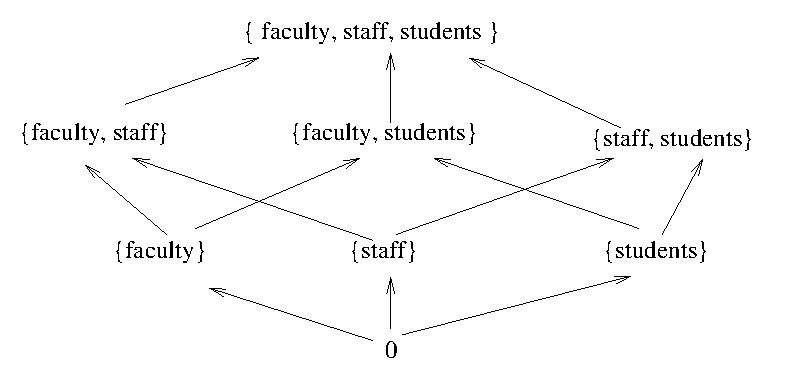
\includegraphics{lattice}}
\end{center}
A file, {\tt payroll.txt}, might have payroll data about students,
faculty, and staff.  
\begin{enumerate}
\item What security class should that file have?  
\item In the lattice model above, can a program with classification
  ``staff'' read such a file?  Why or why not?
\item Faculty may need to read access to student payroll, but may have
  no need to access staff or faculty payroll information.  Suggest how
  the payroll file might be divided into multiple files, and how
  security classes might be assigned, to permit this access granularity.
\end{enumerate}
\vspace{1.25in}
\eprob

\sols{
\vspace{-1.25in}
\begin{answer}
\end{answer}
}

\newpage
\prob{4} Consider the PlayFair cipher below, which has ``Network
Security'' as the key.

\begin{center}
\begin{tabular}{|c|c|c|c|c|}
\hline
N & E & T & W & O \\ \hline
R & K & S & C & U \\ \hline
I & Y & A & B & D \\ \hline
F & G & H & J & L \\ \hline
M & P & V & X & Z \\
\hline
\end{tabular}
\end{center}
\vspace*{0.2in}
\begin{enumerate}
\item Produce the ciphertext corresponding to the plaintext
  ``Encryption is easy''. 
\item Produce the plaintext corresponding to the ciphertext ``BSI EUD
  TGSI NP''
\end{enumerate}
\vspace{1.25in}
\eprob

\sols{
\vspace{-1.25in}
\begin{answer}
\end{answer}
}


\newpage
\section{Design Question: Web Authentication}

George Burdell needs some help designing a Web authentication system for
his new e-Commerce Web site.  He decides to allow his Web site to use
more sophisticated client authentication schemes.  In this problem, you
will evaluate various client authentication mechanisms.

\prob{6} George's first idea is to give a client a
sequence-number-based session identifier when it successfully
authenticates, as follows:

\begin{verbatim}
// secret, not exposed outside of program
unsigned long globalSessionID = 34215;

void success() {
 char redirectURL[256];
 if (authenticated[user]==1) {
   sprintf(redirectURL, "http://burdellbooks.com/%s&sid=%lu", path,
                                globalSessionID) ; 
   /* redirect user to redirectURL */
  ...
  }
}
\end{verbatim}
\noindent
assume that {\tt authenticated[user]} becomes 1 after a user
successfully logs in.

\begin{enumerate}
\item Explain how the above scheme is vulnerable to a brute-force
  guessing attack.  Explain how you might change how the session
  identifier is generated to defend against a brute-force attack.
\item Explain how the above scheme is vulnerable to a replay attack.
  Extend the design of the session identifier to defend against replay
  attacks. 
\end{enumerate}
\eprob


\newpage
\prob{8} George decides instead to place an HTTP cookie on the client
that is applies the {\tt crypt()} function, as follows:
\begin{verbatim}
char* genCookie(char *username) {
  char input[20];
  char cookie[13];

  sprintf(input, "%s%s", username, "secret");
  sprintf(cookie, "%s", crypt(input, "CS"));
  return cookie;
}
\end{verbatim}
\begin{enumerate}
\item How is the above code vulnerable to a buffer overflow?
\item Note that {\tt crypt()} truncates inputs that are longer than
  eight characters.  Explain how you might use a chosen plaintext attack
  to mint authenticators for long usernames.
\item {\em Hard.} Suppose that, as an attacker, you did not know the
  server secret salt ``secret'', but that you could use the server as an
  oracle to produce cookies for arbitrary usernames.  Devise an attack
  to recover the secret.  (There are both exponential and linear time
  attacks.  Full credit for the linear-time attack.)
\end{enumerate}


\eprob

\newpage
\section{Bonus: Anonymous Course Feedback}

{\bf This page is anonymous.}  Rip this off from your exam, and turn it
in separately if you like.  You'll get five points for simply ripping
off the last page of the exam, but I'd prefer if you fill it out and
hand it in in a separate stack.
\vspace{.5in}

What are the things you like most about the course so far?  Anything is
fair game here (topics, course structure, board technique, etc.).
\vspace{1.5in}


What are the things you like least about the course so far?  Again,
anything is fair game.
\vspace{1in}


What topics would you like to see covered?
\vspace{1in}



\label{lastpage}
\end{document}
